\documentclass{IEEEtran}

\usepackage{cite}
\usepackage{amsmath}
\usepackage{amssymb}
\usepackage{url}
\usepackage{graphicx}
\usepackage{booktabs}
\usepackage{microtype}
\usepackage[table]{xcolor}
\usepackage{tikz}
\usetikzlibrary{positioning,arrows.meta,fit,backgrounds}
\usepackage[hidelinks]{hyperref}

\definecolor{PhaseGreen}{RGB}{45,176,150}
\definecolor{PhaseBlue}{RGB}{52,190,255}
\definecolor{PhasePurple}{RGB}{126,87,194}
\definecolor{PhaseOrange}{RGB}{245,166,35}
\definecolor{DeepNavy}{RGB}{11,26,51}

\title{{\LARGE\textbf{Fairness-Aware Routing in Quantum Networks \& Clinical Settings}}\\
{\Large\textit{via Multi-Armed, Contextual, and Informative Bandit Methods}}\\
{\large\texttt{(Approach Writeup)}}}

\author{%
\begin{minipage}{0.48\textwidth}
\begin{center}
{\bf Piter Z. Garcia}\\
\begin{small}
MS Data Science / Decision-Making \& Algorithmic Fairness\\
Rochester Institute of Technology (RIT)\\
{\it pizg8794@g.rit.edu}
\end{small}
\end{center}
\end{minipage}
\hfill
\begin{minipage}{0.48\textwidth}
\begin{center}
{\bf Dr. Daniel Krutz, Travis Desell}\\
\begin{small}
Department of Software Engineering, Data Science\\
RIT Research Advisors\\
{\it dxkvse@g.rit.edu, tjdvse@g.rit.edu}
\end{small}
\end{center}
\end{minipage}%
}

\begin{document}
\maketitle
\vspace{-0.8em}

\section{Approach}

\subsection*{Approach Overview}
This project proposes a fairness-aware sequential routing framework for two settings that at first look unrelated but share the same core problem. In the clinical setting, the system routes patients, tests, and escalation efforts through a diagnostic pathway. COVID-era testing is the clearest example: scarce tests, appointments, and laboratory capacity had to be distributed across communities, and poor distribution quickly became both a fairness failure and a performance failure. In the quantum setting, the system routes entanglement and scarce network resources through candidate paths under probabilistic network conditions. The true common ground is therefore routing under scarcity. In both settings, the system must decide who or what receives the next available opportunity, through which path that opportunity is delivered, and what happens when information is incomplete or uneven across groups.

That shared routing perspective matters because unfair routing also degrades outcomes. In a clinical workflow, groups routed through weaker tests, slower follow-up, or delayed escalation face higher risk of false negatives, delay, and wasted resources. In a quantum workflow, flows repeatedly routed through weaker links or deprioritized during congestion face lower delivery success and worse latency. A second clinical example strengthens the link further: diagnostic systems can begin with missing context when development or validation groups underrepresent minorities or other high-risk populations. The routing process then starts with a weaker picture of the very groups it is supposed to serve. The same pattern appears in bandit-based quantum routing: low-information MABs and weaker contextual setups can ignore relevant routing context, while informative-context methods perform better when that context is restored. The method family is therefore organized as a comparison spectrum rather than a single preferred algorithm. MABs provide a low-information baseline, CMABs test whether side information helps, and iCMABs test whether richer context reduces disparity or simply relocates it.

\subsection*{Shared Domain Model}
The domain model in Figure~\ref{fig:domain_model} is organized into four phases so that the major parts of the approach can be identified quickly and described coherently. Phase 1 defines the routing setting through either a clinical workflow or a quantum network testbed. In the clinical branch, this includes both the allocation of scarce testing and follow-up resources and the evidence-generating environment from which diagnostic signals are produced. In the quantum branch, it includes candidate paths, entanglement resources, and the network state that constrains delivery. Phase 2 forms the observed routing context and isolates the fairness driver of missing, biased, delayed, or uneven information. This is where the motivating examples meet most clearly: a community may receive less access to tests, a subgroup may be represented by weaker measurement assumptions because development data were incomplete, or a routing policy may observe only a partial view of network conditions.

Phase 3 applies the policy family to choose the next routing action, such as test distribution, retesting, escalation, path selection, or resource allocation. MAB, CMAB, and iCMAB are included because the project tests whether fairness and performance improve when relevant context is modeled instead of ignored. Phase 4 records partial feedback, utility, and fairness outcomes, then returns those outcomes to a mitigation and comparison loop. The diagram therefore shows where the routing problem is created, where bias enters through information quality, how actions are chosen, and how outcomes are measured.

\subsection*{Design Rationale}
\noindent\textbf{Why this framing?} The project is designed this way because pairing quantum routing with clinical diagnostic routing creates a stronger argument than studying either one alone. Quantum routing gives the work a forward-looking systems contribution, while clinical routing gives it immediate human relevance. Framing both through fair routing under scarcity makes the research claim clearer: unfairness is not a domain-specific anomaly, but a failure mode that appears when scarce opportunities are repeatedly allocated under imperfect information. The COVID distribution example shows this at the public-health level, and the missing-context example shows that the problem can begin even earlier, at the stage where evidence is created or validated. That same logic gives the quantum branch more than novelty because it suggests that richer routing context may matter for fairness as much as for reward.

\noindent\textbf{Why is this work unique?} This work needs a unified routing framework because the existing landscape is strong in pieces but fragmented in structure. Clinical fairness studies often emphasize offline prediction, static classification, or downstream auditing of pipelines that are already fixed. Routing and network studies, by contrast, often emphasize throughput, reliability, or robustness before fairness becomes a primary design objective. Those lines of work are useful, but they do not directly answer the question this project asks: how unfairness emerges during repeated routing under partial feedback and uneven context quality. A simpler ``use what already exists'' approach would miss that question. A purely offline clinical analysis would not capture sequential decisions such as distribution, retesting, escalation, and deferred follow-up, nor would it capture how missing context from under-representative development can propagate into later decisions. A purely technical routing study would miss the direct human stakes that make fairness failures easy to interpret.

\noindent\textbf{Why is this approach stronger?} This approach is better than narrower alternatives because it explains more and tests more. A one-domain study would produce a smaller claim. By bringing the two domains together, the project shows that the same routing logic can expose fairness failures in both people-centered and infrastructure-centered settings. It is also better than a single-model comparison because the method spectrum itself is part of the contribution. The project is not trying to declare one best algorithm in the abstract. It is testing whether low-information, contextual, and richer-context routing methods change the fairness-performance tradeoff in different ways. That makes the analysis more defensible and also explains why iCMABs matter here specifically: if they consistently outperform weaker alternatives, the result supports the claim that missing context is a central fairness-and-performance driver across both testbeds.

\subsection*{Implementation Logic}
\noindent\textbf{Why this design and implementation?} The major design decisions follow directly from the research question. The clinical branch is simulation-first by design so that missingness, delay, noise, subgroup-sensitive measurement quality, intervention cost, and distribution constraints can be controlled directly instead of being inherited from a fixed retrospective dataset. That makes it possible to instantiate both motivating clinical examples inside one testbed: unfair routing of scarce tests and follow-up resources, and missing-context conditions caused by weaker representation of some groups in the evidence-generating process. The quantum branch builds on a routing and resource-allocation setting so that the second domain remains technically credible and tied to real constraints such as probabilistic links, congestion, and limited entanglement resources.

The implementation plan is also deliberate. Both testbeds are exposed through a shared policy interface so that the same family of methods can be evaluated under comparable rounds. Reward and fairness metrics remain domain-specific but structurally aligned. The framework records measures such as diagnostic accuracy, intervention delay, routing access, and resource cost in the clinical setting, and delivery success, latency, and service-equity gaps in the quantum setting. Those outcomes are logged per step and summarized over time so that the project can distinguish temporary unfairness during learning from persistent unfairness after longer runs. Reproducibility is supported through fixed random seeds, explicit configuration files, modular experiment runs, and at least one mitigation mechanism evaluated within the same loop.

\noindent\textbf{Connecting decisions to the domain model.} Every major decision in the project maps back to the domain model. The simulation or network testbed corresponds to Phase 1 because that is where the routing setting is created. The choice to model missing, delayed, biased, or uneven information explicitly corresponds to Phase 2 because that is where fairness pressure enters the decision process and where the clinical and quantum parallels become most visible. The choice to compare multi-armed, contextual, and informative-context methods corresponds to Phase 3 because that is where the routing policy converts imperfect information into action. The logger, fairness metrics, and mitigation mechanism correspond to Phase 4 because that is where the framework measures outcomes and tests whether the routing process can be improved. The COVID-style distribution example explains how scarcity and access create unfair routing pressure in the clinical branch, while the missing-context example explains why iCMAB-style informational gains matter in both branches. That relationship between design decision and domain model is what makes the approach cohesive rather than simply ambitious.

\vspace{-0.25em}
{\footnotesize\begin{thebibliography}{9}\setlength{\itemsep}{0em}
\bibitem{garcia2025equitable_bioinformatics}
Garcia, P. Z. Equitable Bioinformatics: Enhancing Diagnostic Decision-Making through {RNA}
and Biomarker Data. Course paper (ISTE 780 Phase 4), Rochester Institute of Technology,
2025.
\bibitem{garcia2026threat_aware_quantum_routing}
Garcia, P. Z. Threat-Aware Evaluation of Quantum Entanglement Routing and Qubit Allocation
via Hybrid Contextual Bandits. Unpublished manuscript (GA-Work internal draft), Rochester
Institute of Technology, 2026.
\end{thebibliography}}

\clearpage
\onecolumn
\begin{center}
\resizebox{0.98\textwidth}{!}{%
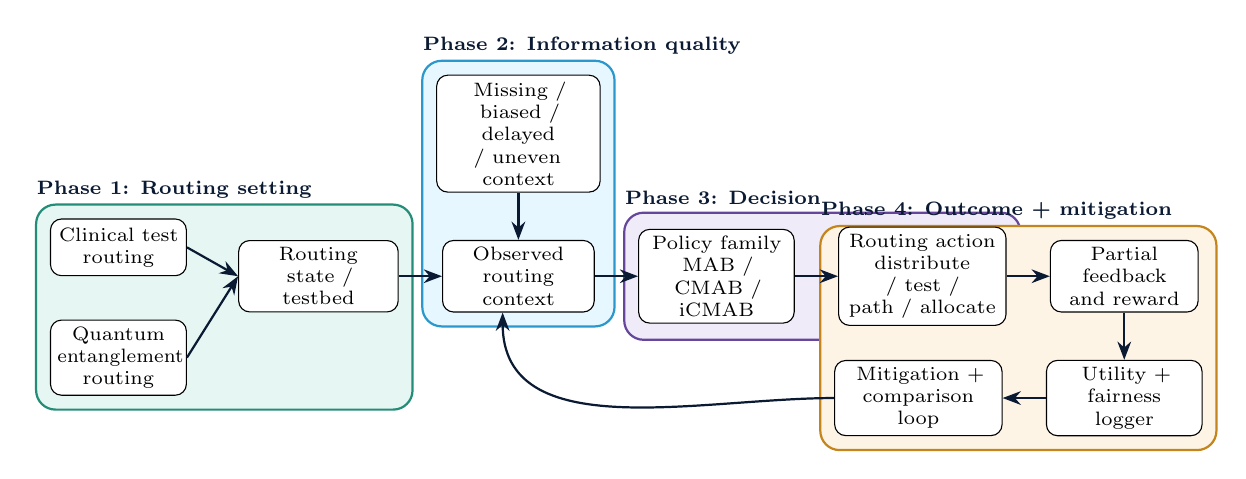
\begin{tikzpicture}[
font=\scriptsize,
box/.style={draw, rounded corners=4pt, align=center, text width=1.55cm, minimum height=0.72cm, inner sep=2.5pt, fill=white},
arr/.style={-Stealth, thick, draw=DeepNavy},
phase/.style={draw, rounded corners=7pt, inner sep=5pt, thick},
phaselabel/.style={font=\scriptsize\bfseries, text=DeepNavy, anchor=west}
]
\node[box] (clin) {Clinical test\\routing};
\node[box, below=0.55cm of clin] (quant) {Quantum\\entanglement\\routing};
\node[box, right=0.65cm of clin.south east, anchor=west, text width=1.85cm] (env) {Routing\\state /\\testbed};
\node[box, right=0.55cm of env, text width=1.75cm] (ctx) {Observed routing\\context};
\node[box, above=0.60cm of ctx, text width=1.90cm] (deg) {Missing / biased /\\delayed / uneven\\context};
\node[box, right=0.55cm of ctx, text width=1.80cm] (pol) {Policy family\\MAB / CMAB / iCMAB};
\node[box, right=0.55cm of pol, text width=1.95cm] (act) {Routing action\\distribute / test /\\path / allocate};
\node[box, right=0.55cm of act, text width=1.70cm] (fb) {Partial feedback\\and reward};
\node[box, below=0.60cm of fb, text width=1.80cm] (log) {Utility + fairness\\logger};
\node[box, left=0.55cm of log, text width=1.95cm] (mit) {Mitigation +\\comparison loop};

\begin{scope}[on background layer]
\node[phase, fill=PhaseGreen!12, draw=PhaseGreen!80!black, fit=(clin)(quant)(env)] (p1) {};
\node[phase, fill=PhaseBlue!12, draw=PhaseBlue!80!black, fit=(ctx)(deg)] (p2) {};
\node[phase, fill=PhasePurple!12, draw=PhasePurple!80!black, fit=(pol)(act)] (p3) {};
\node[phase, fill=PhaseOrange!12, draw=PhaseOrange!80!black, fit=(fb)(log)(mit)] (p4) {};
\end{scope}

\node[phaselabel] at ([xshift=-0.10cm,yshift=0.18cm]p1.north west) {Phase 1: Routing setting};
\node[phaselabel] at ([xshift=-0.10cm,yshift=0.18cm]p2.north west) {Phase 2: Information quality};
\node[phaselabel] at ([xshift=-0.10cm,yshift=0.18cm]p3.north west) {Phase 3: Decision};
\node[phaselabel] at ([xshift=-0.10cm,yshift=0.18cm]p4.north west) {Phase 4: Outcome + mitigation};

\draw[arr] (clin.east) -- (env.west);
\draw[arr] (quant.east) -- (env.west);
\draw[arr] (env) -- (ctx);
\draw[arr] (deg) -- (ctx);
\draw[arr] (ctx) -- (pol);
\draw[arr] (pol) -- (act);
\draw[arr] (act) -- (fb);
\draw[arr] (fb) -- (log);
\draw[arr] (log) -- (mit);
\draw[arr] (mit.west) to[out=180,in=270] ([xshift=-0.20cm]ctx.south);
\end{tikzpicture}%
}
\par\vspace{0.5em}
\small\textbf{Figure 1.} Color-coded shared domain model. The same four phases support both settings while preserving domain-specific meanings for routing state, action, reward, and fairness metrics, including scarce test distribution, missing clinical context, and quantum entanglement routing.
\label{fig:domain_model}
\end{center}

\end{document}
